\documentclass[border=10pt]{standalone}
\usepackage[svgnames]{xcolor}
\usepackage{amsmath}
\usepackage{pgfplots}
\pgfplotsset{compat=newest}
\usepackage[sfdefault]{FiraSans}
\usepackage{FiraMono}
\renewcommand*\familydefault{\sfdefault}
\begin{document}
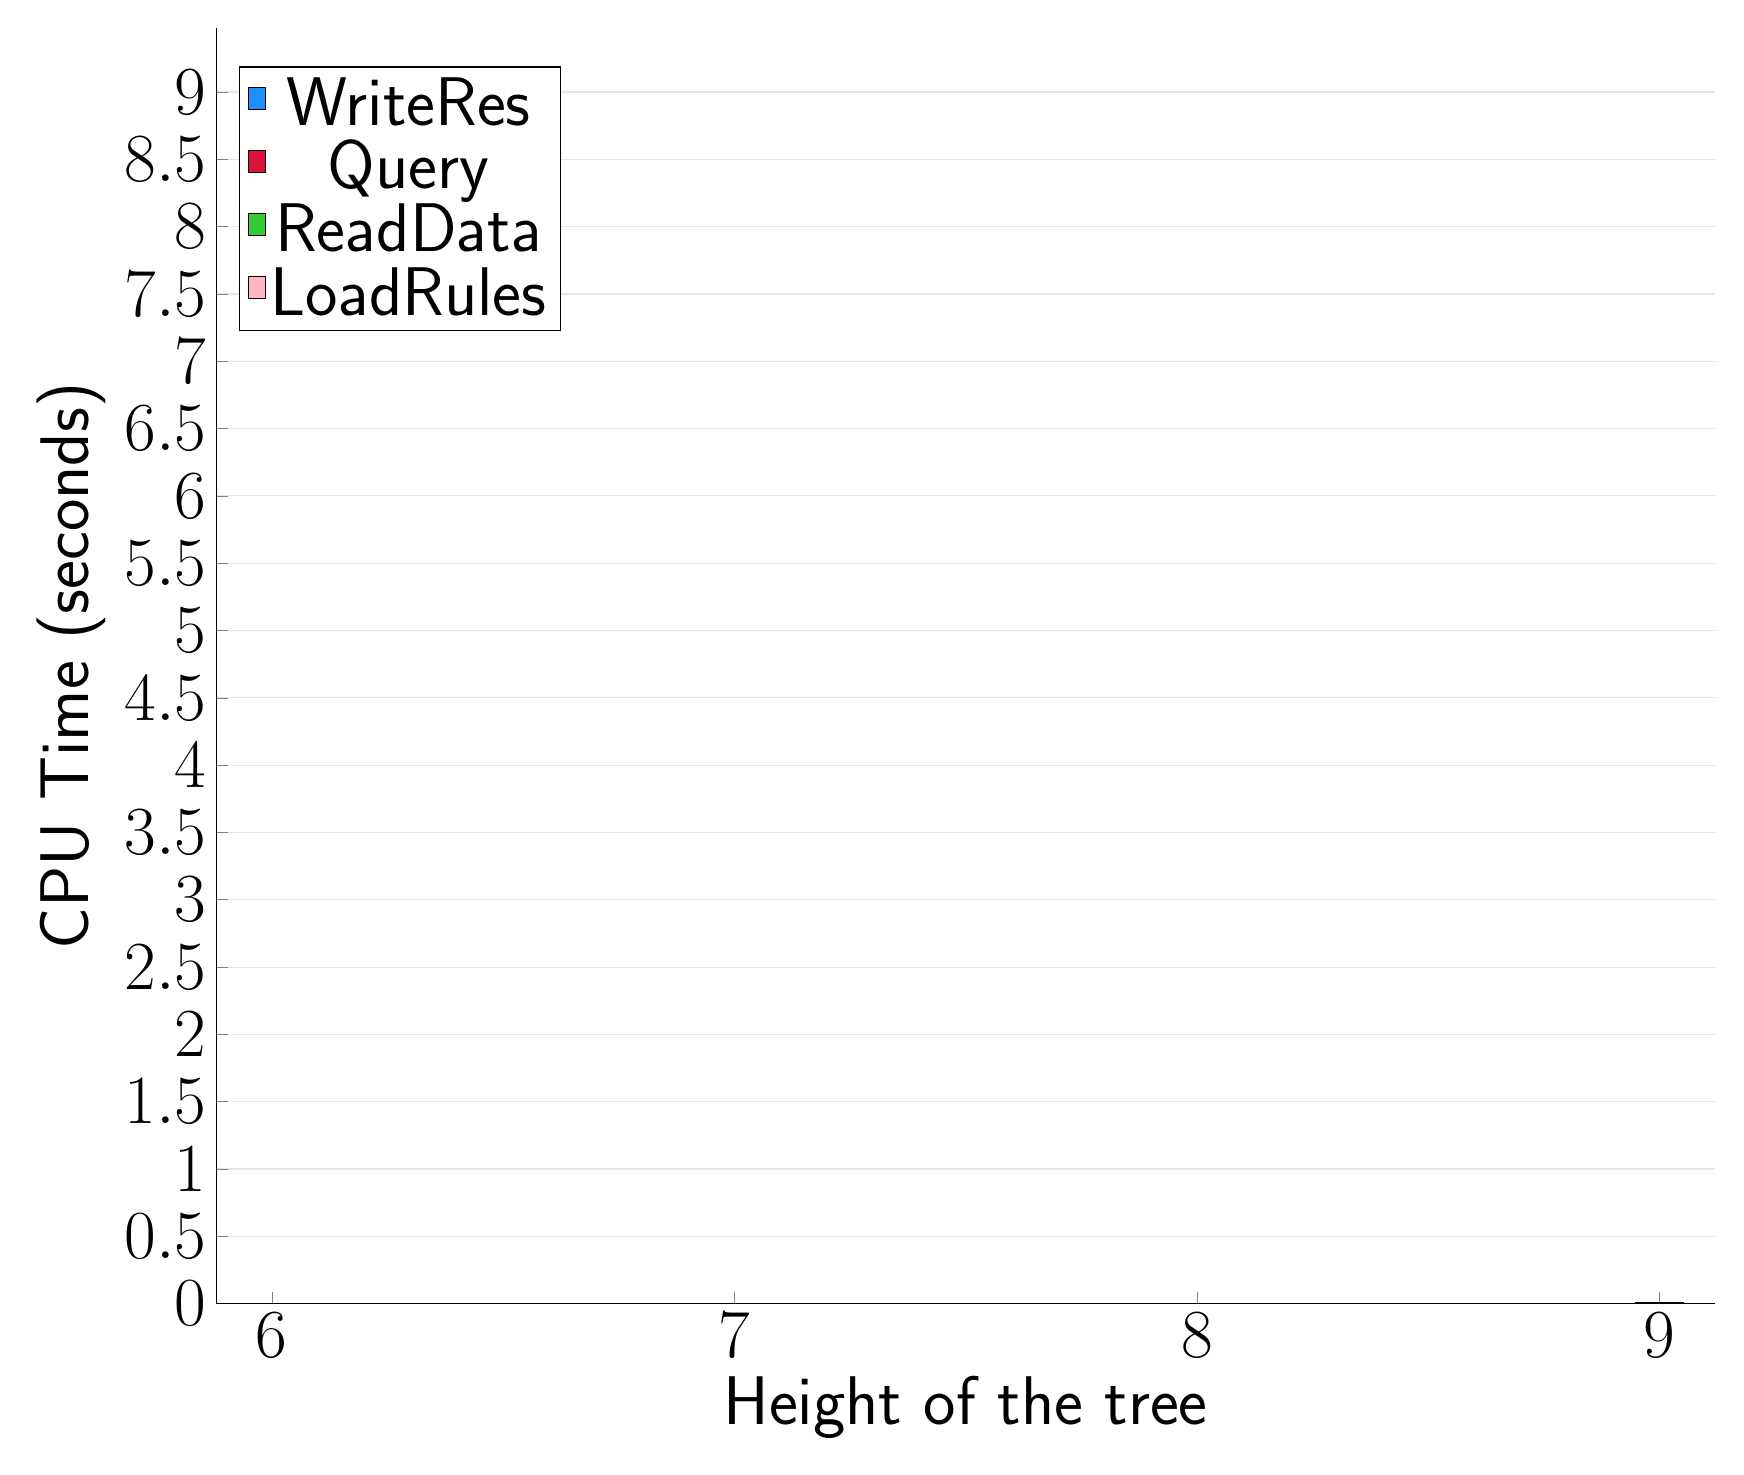
\begin{tikzpicture}
\begin{axis}[
   ybar stacked,
   width=1.7\textwidth,
   bar width=0.6cm,
   ymajorgrids, tick align=inside,
   major grid style={draw=gray!20},
   xtick=data,
   ymin=0, ymax=9.474,
   axis x line*=bottom,
   axis y line*=left,
   enlarge x limits=0.04,
   legend style={
       at={(0.23, 0.97)},
       anchor=north east,
       legend columns=1,
       font=\Huge,
   },
   ylabel={CPU Time (seconds)},
   xlabel={Height of the tree},
   label style={font=\Huge},
   tick label style={font=\Huge},
]
\addlegendimage{fill=DodgerBlue, draw=black, line width=0.2pt}
\addlegendentry{WriteRes}
\addlegendimage{fill=Crimson, draw=black, line width=0.2pt}
\addlegendentry{Query}
\addlegendimage{fill=LimeGreen, draw=black, line width=0.2pt}
\addlegendentry{ReadData}
\addlegendimage{fill=LightPink, draw=black, line width=0.2pt}
\addlegendentry{LoadRules}
\addplot +[fill=LightPink, draw=black, line width=0.55pt] coordinates {
(6, 0.0005594000000000003)
(7, 0.0005519999999999995)
(8, 0.0005565999999999995)
(8, 0.0005484000000000002)
(8, 0.0005575999999999995)
(9, 0.0005519999999999998)
(9, 0.0005548)
(9, 0.0005568)
(9, 0.0005566000000000006)
(9, 0.0005512000000000002)
};
\addplot +[fill=LimeGreen, draw=black, line width=0.55pt] coordinates {
(6, 0.0001728000000000002)
(7, 0.0002232000000000006)
(8, 0.0003250000000000002)
(8, 0.00031899999999999984)
(8, 0.00032400000000000104)
(9, 0.0005245999999999998)
(9, 0.0005218)
(9, 0.0005182000000000002)
(9, 0.0005183999999999994)
(9, 0.0005323999999999994)
};
\addplot +[fill=Crimson, draw=black, line width=0.55pt] coordinates {
(6, 3.259999999999998e-05)
(7, 6.159999999999986e-05)
(8, 0.00013320000000000042)
(8, 0.0001289999999999996)
(8, 0.0001339999999999994)
(9, 0.000291800000000001)
(9, 0.00028440000000000003)
(9, 0.0002819999999999996)
(9, 0.00029160000000000064)
(9, 0.0002980000000000008)
};
\addplot +[fill=DodgerBlue, draw=black, line width=0.55pt] coordinates {
(6, 0.00027280000000000023)
(7, 0.0005932000000000003)
(8, 0.0013193999999999994)
(8, 0.0013376000000000004)
(8, 0.0013130000000000006)
(9, 0.002993599999999999)
(9, 0.0029736000000000007)
(9, 0.0029914000000000004)
(9, 0.0030071999999999994)
(9, 0.002954799999999999)
};
\end{axis}
\end{tikzpicture}

\end{document}
